\chapter{Designing and Implementing the OurPlace Platform}
\label{chap:Design}

Following the engagements covered in Chapter \ref{chap:DesignSpace}, I decided to iterate upon the Park:Learn prototype application. With the aim of creating an application which could be utilised in formal and informal learning contexts, I examined previous mobile learning research (summarised in Chapter \ref{chap:MobileLearning}) to produce a number of design goals for the technology. This application would also aim to follow the implications for design (as described in section \ref{sec:SuggestionsCivicLearning}) derived from the findings of the previous exploratory study. This chapter describes the design goals for the technology, why those goals were chosen, a detailed overview of the application itself and how it evolved over the course of the remainder of the project. Much of the work covered by this chapter was peer-reviewed and published at MobileHCI 2018 \citep{Richardson2018}, with the paper being co-authored by Doctors Pradthana Jarusriboonchai, Kyle Montague and Ahmed Kharrufa. 

\section{Technology Design Goals}

Based on the findings of previous works and the design engagements covered in Chapter \ref{chap:DesignSpace}, we produced several design goals (DGs). This section describes each design goal and the rationale behind choosing them.

% reference like this: (addresses \hyperref[DG1]{DG1})

\subsection*{ DG1: Utilize local places and communities as learning resources }
\phantomsection
\label{DG1}

This first goal is that the final technology should support greater utilisation of local places (e.g. parks, buildings, towns, rooms, etc) and the communities which surround, inhabit and have built relationships with them as learning resources. This primarily relates to the previously discussed Park:Learn studies, during which we found that places' stakeholders can offer not only a diverse knowledge base, but also a large variety of motivations, aspirations and tensions related to place. We suggested that mobile learning technologies might be able to make use of these social infrastructures, by giving places’ stakeholders a platform for sharing their values through designing and sharing learning activities in authentic contexts \citep{Richardson2017}. This would not only support learners in situating their learning activities within authentic physical environments, but might also introduce them to new communities of practice which they may enter and develop an expertise through interactions with them \citep{lave1991situated}.

\subsection*{ DG2: Support seamless outdoor and classroom use }
\phantomsection
\label{DG2}

As noted by Sharples, mobile learning does not necessarily always take place in one context, or even one fixed level of formality \citep{Sharples2013}. He presents mobile learning as taking place on a linear spectrum: from formal, classroom and curriculum-based learning activities, to ones are informal, creative and \textit{mobile} \ref{fig:learningContextDimension}. However, while these contexts are different, they can still be connected---Kuh argues that learning experiences across contexts can be bound into a `seamless learning' narrative \citep{Kuh1996}. In order to support this seamless use across contexts, our design should encompass as many of Wong and Looi's `desirable dimensions' of seamless learning as possible \citep{Wong2011} (all ten dimensions are listed in section \ref{sec:Seamless}). Multiple examples of seamless mobile learning applications which adhere to some (or all) of these dimensions already exist. For example, Zydeco supports the use of multiple types of devices across multiple locations (classrooms and museums), utilising both digital and physical learning resources \citep{kuhn2011}.

\subsection*{ DG3: Support a variety of pedagogical approaches and stakeholder requirements }
\phantomsection
\label{DG3}

The final `desirable dimension' listed by Wong and Looi is that seamless mobile learning technologies should encompass multiple pedagogical models, as a diversity of learning experiences requires the deployment of different learning models \citep{Wong2011}. For example, the learning theory of constructionism and project-based learning pedagogies (as covered in section \ref{sec:ConstructionismPBL}) have different requirements to more traditional classroom teaching methods. Sessions within these pedagogies will often have different goals, with the intended outcomes also changing according to the stakeholders' agenda (e.g. teachers may want to be able to provide evidence of students' learning, while park rangers and volunteers may want to promote place-making in an attempt to nurture stewardship and volunteerism \citep{Richardson2017}). As such, our technology needs to be flexible enough to support different goals, learning processes and intended outcomes, ideally without relying heavily on additional tools.

\subsection*{ DG4: Support a wide range of user ages and technical expertise }
\phantomsection
\label{DG4}

While it has almost become a truism that children are frequently technologically adept, care still needs to be taken to support age and ability groups who may struggle with reading or typing large quantities of text (as shown to be an issue in MyArtSpace \citep{Vavoula2009} and deliberately avoided in Zydeco \citep{kuhn2011}). Furthermore, engaging with a large variety of place stakeholders means that older age groups---who may not be as technologically literate---may wish to use the technology. Our technology design will therefore strive to minimise (or provide alternatives to) large amounts of typing, and, as suggested by Land, attempt to support a range of learner ages and reading abilities through the use of simple, varied but semantically consistent visual interfaces \citep{Land2015}.

\subsection*{ DG5: Support learning and reflection in authentic learning contexts }
\phantomsection
\label{DG5}

Our observations in the initial engagements (as well elements found in prior work, such as in Mobilogue \citep{Giemza2013}) demonstrated that giving students greater control and opportunities for creativity can act as a motivating factor. As such, our design aimed to utilise interaction methods on mobile devices which support student creativity and control in authentic learning environments. That said, while not all mobile learning projects made use of the learner's context as a learning environment or resource \citep{Frohberg2009}, even fewer promote learner reflection within the authentic learning environment. For example, MyArtSpace \citep{Vavoula2009} and Sense-It \citep{Sharples2017} encourage learners to use the technology to collect data or take brief notes and observations, rather than engage in in-depth reflection in-situ. This is certainly useful, and should have a place in the final design. However, we wanted our design to also support immediate reflection from the learner, without the need to return to the classroom. This level of immediacy should also apply to activity creation and data collection, in an attempt to minimise the learner being distracted from authentic engagement with the learning context. 

\subsection*{ DG6: Support mobile learning in resource-limited schools }
\phantomsection
\label{DG6}

As discussed in sections \ref{sec:DigitalCivics} and \ref{sec:ParkContext}, the UK as a whole is enduring an extended period of austerity and local authorities have had to cut funding wherever possible. As a result, many schools have become resource-limited and may struggle to justify spending money on having more smart mobile devices for classroom use, despite them becoming more affordable and fashionable within education. While our final software design will require the use of a smartphone or tablet, it must take steps to minimise the financial strain placed upon schools in its use. The design should: require minimal teacher time to set up and use, as well as access and download student work; support the sharing of devices between multiple students, either through group work or the ability to save and clear progress to allow another student to start activities afresh (as seen in Mobilogue \citep{Giemza2013}); and support the offline caching of data, allowing teachers to pre-load content in the classroom prior to trips, or queuing student work for later upload (avoiding expensive 4G mobile data contracts).

\section{An Overview of ParkLearn and OurPlace}

ParkLearn, the prototype application discussed in Chapter \ref{chap:DesignSpace}, was further developed to meet these design goals. While the early version was created as a simple proof of concept and acted as a technology probe, later versions featured far greater functionality. This section will detail the application: its features, its implementation, and how it evolved over time into the later OurPlace app. As the two versions are extremely similar, for the sake of clarity `OurPlace' will be used as the application's name for the rest of this chapter. Significant differences in the two applications' features or implementations will be noted explicitly.

The main screen of the OurPlace app consists of two main sections, separated by tabs: `Highlights', which shows public content created by all users, and `My Creations', which lists the content created by the current user. This section details the nature of this content, how it is experienced by learners, how users can create their own, and how it can be shared with others.

\subsection{The Anatomy of an Activity}
\label{sec:ActivityOverview}
Core to the OurPlace application is the concept of `Activities'. In terms of user interaction, they are the more or less the same as the ones introduced in the prototype ParkLearn application, based on the original jigsaw workshop activity (Figure \ref{fig:rangerJigsaw}). While the Activities in the prototype version were hard-coded into the application, later versions allowed users to create their own Activities, or complete other people's. They are delivered to the mobile app by the remote server in the standard JSON data format (see section \ref{sec:ImplementationWeb}), allowing for the app to allow users to discover and open Activities in numerous ways (see section \ref{sec:SharingActivities}).

Activities are typically based on a particular topic, location or subject (e.g. `\textit{Exploring the Rose Garden}'). Each OurPlace Activity must feature a title and a short (up to 150 characters) description, which gives the learner some insight into what the Activity will be about (Figure \ref{fig:ActivityExample}). Additionally, Activity creators may choose to include an image to represent the Activity: this will appear on the application's feeds, and at the top of the main Activity screen. The application supports taking this image directly through the device's camera, or the use of pre-existing images from the user's photo gallery (allowing users to select images they prepared earlier, or downloaded from the Internet). By allowing both options, activity creators are able to either create their Activities within the relevant physical context (addresses \hyperref[DG5]{DG5}) or remotely, which may be easier if preparing for a future school trip (addresses \hyperref[DG6]{DG6}).

\begin{figure*}
  \centering
  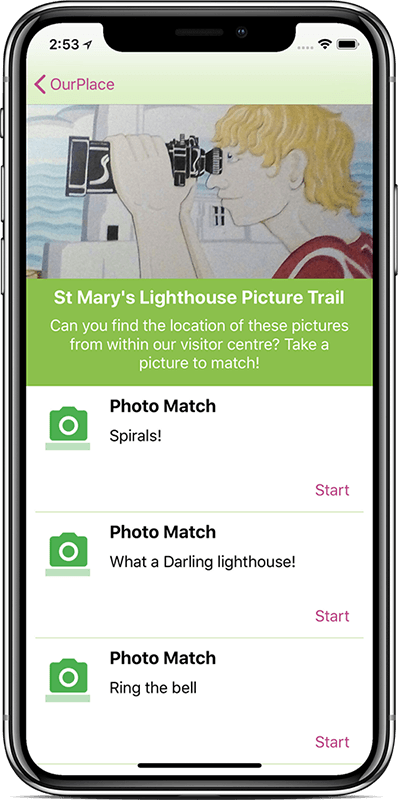
\includegraphics[width=0.85\columnwidth]{images/chapter05/activity.png}
  \caption[A simple OurPlace Activity]{ A simple Activity in the OurPlace iPhone app. The Activity's image, title and description appear at the top, with Tasks underneath. The Task Type of each Task is made known to the user by displaying its name and icon. The screen can scroll vertically if there are more Tasks than can be displayed at once. }~\label{fig:ActivityExample}
\end{figure*}

Each Activity must also feature at least one `Task'. Tasks are modular, and each one centres around a single user interaction (e.g. `\textit{Take a Photo}'). A large number of variations (`Task Types') of Tasks are available, supporting a berth of different interactions (addresses \hyperref[DG3]{DG3}). Section \ref{sec:TaskTypes} describes all of the different Task Types available in OurPlace (note that `\textit{Scan the QR Code}' was introduced in OurPlace, and was not available in ParkLearn). An Activity can have an unlimited number of Tasks, and the learner is able to complete them in any order.

As noted in Chapter \ref{chap:DesignSpace}, each of these interactions were chosen either because they put an element of creative control into the hands of the learner (\textit{Take a Photo, Draw a Picture, Draw on Photo, Record Video, Record Audio}) (addresses \hyperref[DG5]{DG5}), took advantage of the devices’ hardware capabilities across different contexts (\textit{Listen to Audio, Map Marking, Location Hunt, Scan the QR Code}) (addresses \hyperref[DG2]{DG2}), emulated features of the learning materials already in use by teachers and park rangers (\textit{Information, Multiple Choice, Text Entry}) (addresses \hyperref[DG3]{DG3}), or a combination of all of the above.

\begin{figure*}
  \centering
  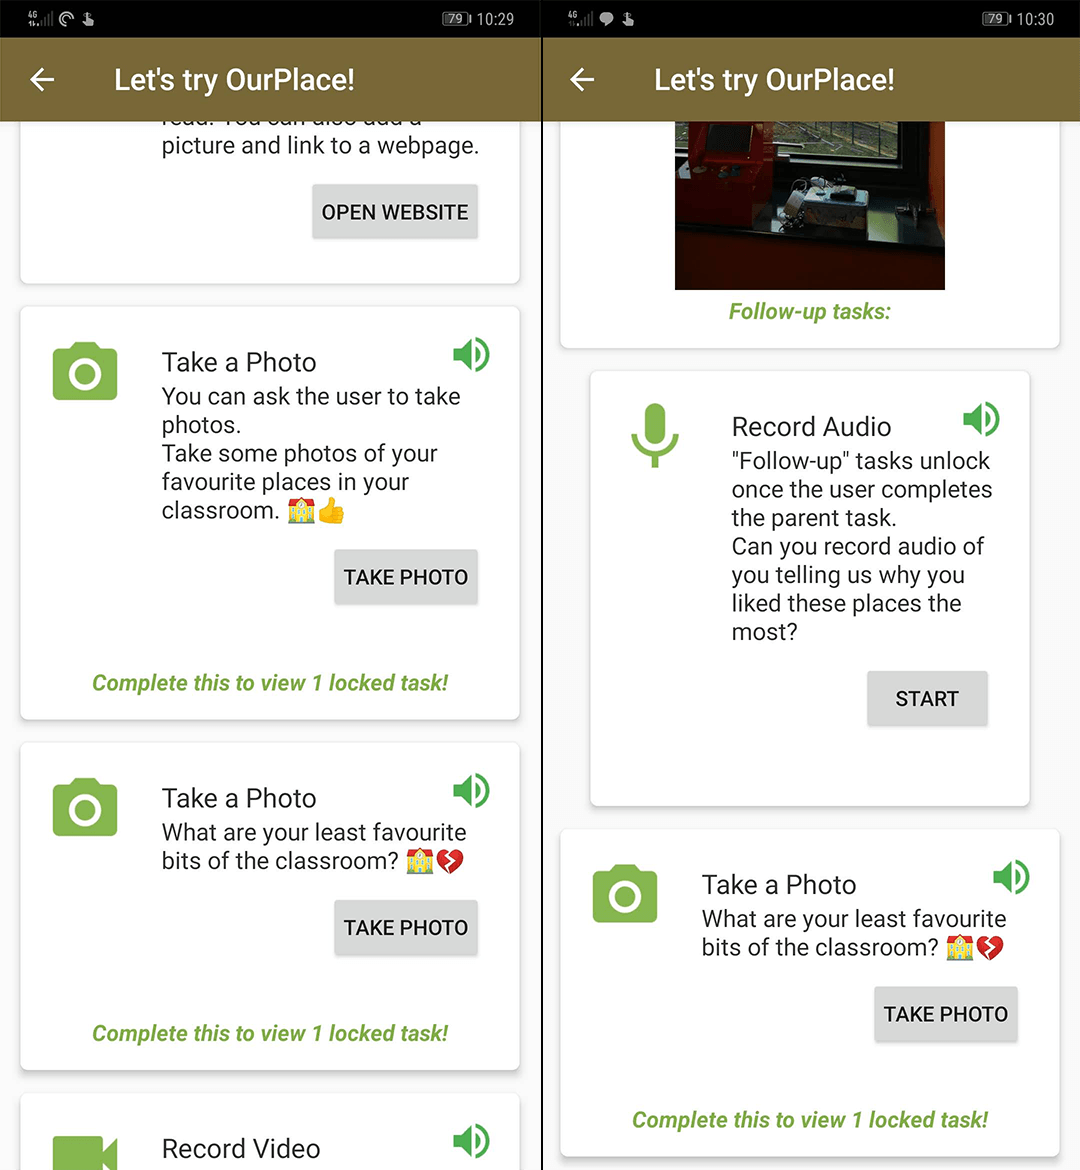
\includegraphics[width=0.8\columnwidth]{images/chapter05/FollowUpTasks.png}
  \caption[Follow-Up Task example]{An example of how Follow-Up Tasks work. Completing `parent' Tasks (left) makes any Follow-Up Tasks they might have available to the learner. Follow-Up Tasks are listed below the parent, and appear on slightly smaller cards to make them visually distinct (right). }~\label{fig:FollowUpTasks}
\end{figure*}

The OurPlace app also features the concept of `Follow-Up Tasks', which were not available in ParkLearn. Follow-Up Tasks act as children to a chosen parent Task, only becoming available when the parent has been marked as completed by the system (Figure \ref{fig:FollowUpTasks}). For example, a Task might ask the learner to take a picture of the item in a museum they found most interesting, and then a Follow-Up Task could ask them to record an audio clip of them explaining what was interesting about it. Having this ability allows Activity designers to encourage students to reflect through the application, while still in the authentic learning environment (addresses \hyperref[DG5]{DG5}). In order to make learners aware of locked Follow-Up Tasks, a `\textit{Complete this to view X locked tasks!}' message is displayed upon the parent Task (Figure \ref{fig:FollowUpTasks}, left). Once the parent Task has been completed, the message changes to `\textit{Follow-Up Tasks:}' and the child Tasks are listed below the parent (Figure \ref{fig:FollowUpTasks}, right). To make the Follow-Up Tasks visually distinct, they appear on slightly smaller cards in the app's interface than their parents. Once completed, Tasks cannot be `uncompleted' (e.g. by deleting all taken photos), meaning that unlocked Follow-Up Tasks will remain available unless the Activity's progress is completely reset.


\subsection{Overview of Task Types}
\label{sec:TaskTypes}
Below are all of the Task Types available to users creating Activities in the OurPlace application. Unless noted otherwise, the functionality of each Task Type was identical between ParkLearn and OurPlace. All Task Types contain a some sort of textual description or instruction, with a `text to speech' button which reads the description aloud when pressed. If a Task has an interaction for the learner to perform, it will either be assigned to an `action button' (e.g. `TAKE PHOTO' and `START' in Figure \ref{fig:FollowUpTasks}) which will navigate to a new screen in the app, or take place on the Activity's main screen (e.g. Multiple Choice and Text Entry in Figure \ref{fig:TaskTypes3}). 

\begin{figure*}
  \centering
  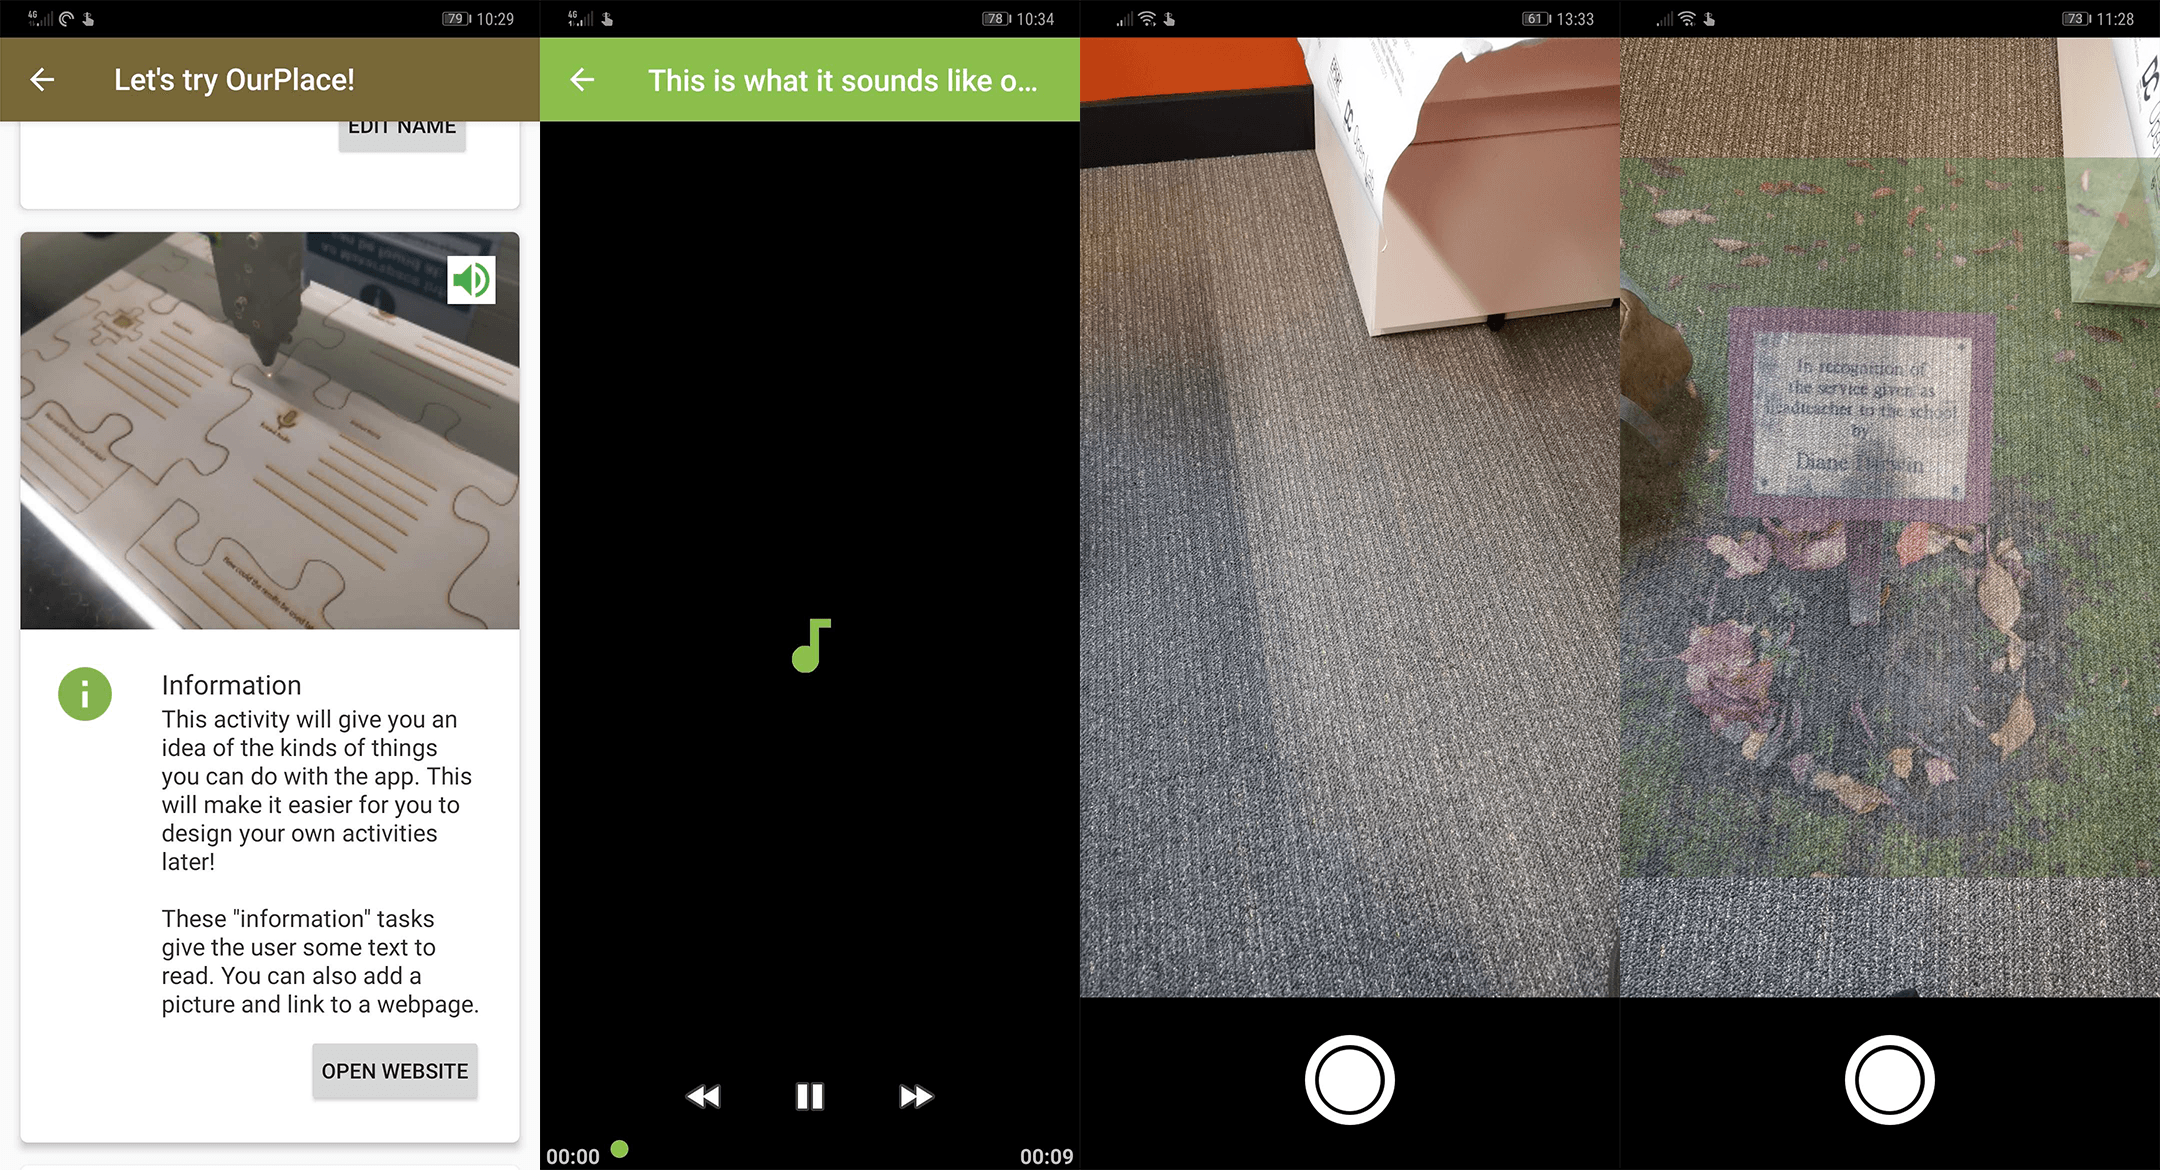
\includegraphics[width=1\columnwidth]{images/chapter05/tasktypes1.png}
  \caption[Task Types (part 1)]{Task Types (left to right): a) Information; b) Listen to Audio; c) Take a Photo; d) Photo Match}~\label{fig:TaskTypes1}
\end{figure*}

\subsubsection*{Information}
One of the simple Task Types, this presents the learner with a piece of text to read. Optionally, the Activity author can also choose to include an image to accompany the text, as well as a hyperlink to a related web page. If included, the hyperlink is assigned to the Task's action button, which will open the address in the device's default web browser when pressed (Figure \ref{fig:TaskTypes1}.a). because they are passive (and the action button is optional), Information Tasks are marked as completed by default, meaning any Follow-Up Tasks are immediately visible.

\subsubsection*{Listen to Audio}
The learner is given an audio recording to listen to. Tapping the Task's action button will open up a media player screen, where the audio file plays on a loop until closed (Figure \ref{fig:TaskTypes1}.b). The Task is marked as completed when the media player is closed. The original ParkLearn application was slightly different, in that the audio played from the Activity's main screen, with a simple `stop' button being shown on a pop-up.
    
\subsubsection*{Take a Photo}
The learner is asked to take one or more photos of a subject. The action button opens up a simple camera screen (Figure \ref{fig:TaskTypes1}.c). While applications would usually use the device's default camera application, the app's other camera-related Task Types have more complex requirements requiring custom solutions, and the custom camera screen is also used here for the sake of consistency. When a photo is taken, the camera closes and returns to the Activity screen. Multiple photos can be taken, and they are listed below the Task's action button (Figure \ref{fig:MediaViewer}.a). Tapping one of these will open it in the media viewer screen, where the user can see a larger view of the photo and can delete it by tapping a bin icon (Figure \ref{fig:MediaViewer}.b). The original ParkLearn app did not have this media viewer screen, however unwanted images could be deleted by tapping and holding them.

\begin{figure*}
  \centering
  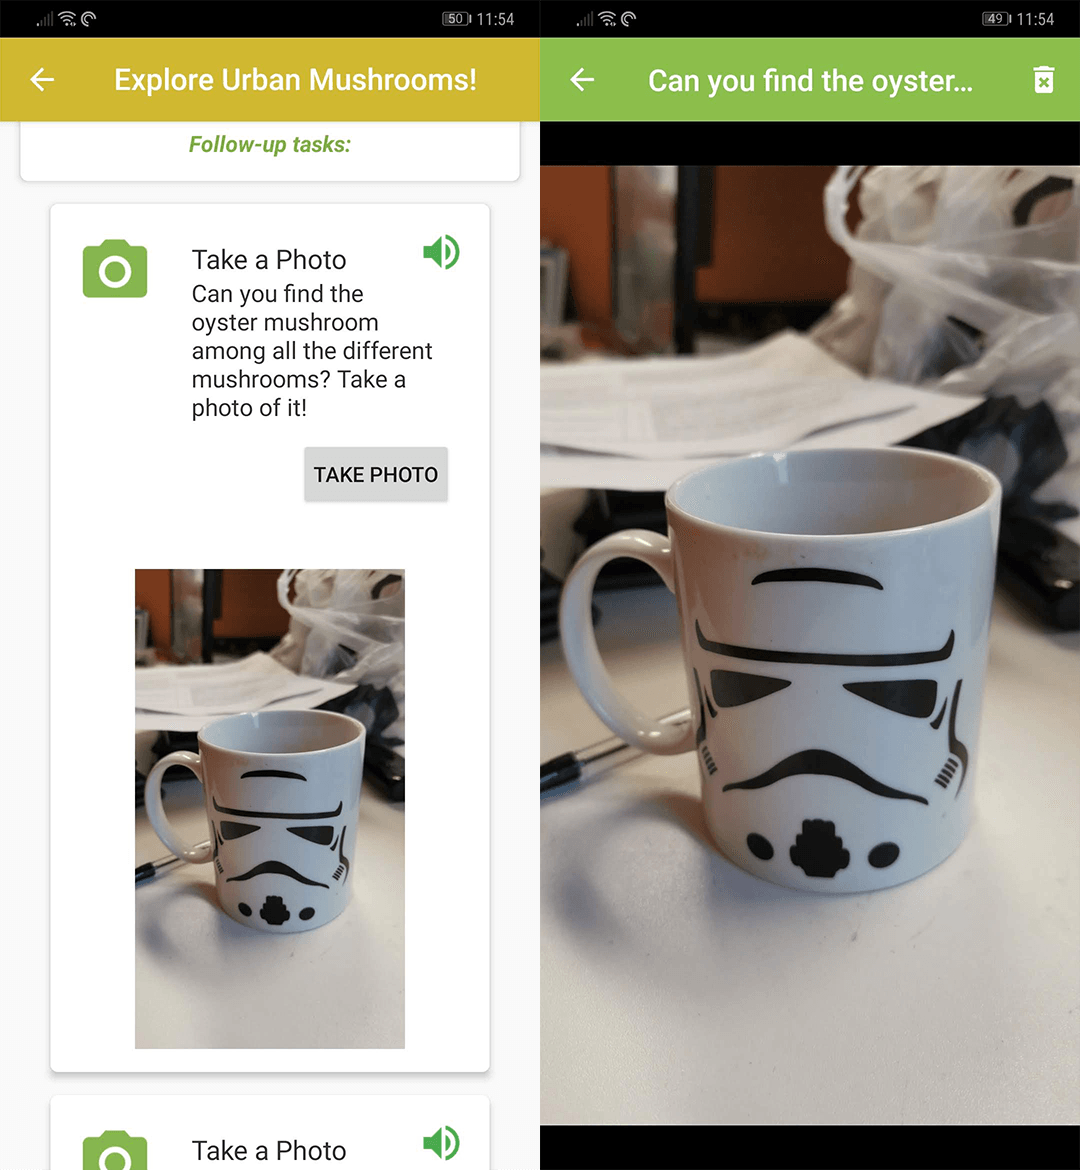
\includegraphics[width=0.65\columnwidth]{images/chapter05/mediaViewer.png}
  \caption[OurPlace's media viewer]{(left to right): a) Resulting images from `Take a Photo' are listed below the Task on the Activity screen. b) Tapping one opens it on the media viewer screen, where the option to delete the item is available.}~\label{fig:MediaViewer}
\end{figure*}

\subsubsection*{Photo Match}
This is similar to `Take a Photo', in that the learner is asked to take one or more photos of a subject. However, the camera screen shows a semi-transparent overlay of another image on top of the camera feed (Figure \ref{fig:TaskTypes1}.d). The Activity author provides an image of their own choosing (e.g. a photo they have taken, or downloaded from the Internet). Viewing and deleting resulting images is handled the same as in Take a Photo.

\begin{figure*}
  \centering
  \includegraphics[width=1\columnwidth]{images/chapter05/tasktypes2.png}
  \caption[Task Types (part 2)]{Task Types (left to right): a) Draw a Picture; b) Draw on Photo; c) Record Video (rotated); d) Record Audio}~\label{fig:TaskTypes2}
\end{figure*}

\subsubsection*{Draw a Picture}
The learner is asked to draw a picture, using a basic painting interface which is launched by tapping the Task's action button. A wide variety of colours can be selected using the selector at the top of the screen, and drawn onto a blank white canvas (Figure \ref{fig:TaskTypes2}.a). Tapping the save icon will save the drawing as a JPEG file and return to the Activity screen, where it can be viewed/deleted in the same way as photo files. Multiple drawings can be made.

\subsubsection*{Draw on Photo}
Functionally the same as `Draw a Picture', however the blank white canvas is replaced by a supplied image (Figure \ref{fig:TaskTypes2}.b). The Activity author can either provide an image of their own choosing (e.g. a photo they have taken, or downloaded from the Internet), or---if this is a Follow-Up Task to an appropriate parent, such as a Take a Photo or Photo Match---have the overlay be one of the images taken by the learner in the parent Task. Images can be viewed and deleted in the same way as other photos and drawings.

\subsubsection*{Record Video}
Learners are asked to record a video of a subject using the camera, which is launched by tapping the action button. The camera screen is locked in the landscape orientation, and features a help button which will show the Task's description/instruction when pressed (Figure \ref{fig:TaskTypes2}.c). Recording starts when the shutter button is tapped, at which point the button turns red. To minimise storage issues, a custom video recorder screen was needed, which capped recordings at 10 minutes in length and at a 720p resolution. When the shutter button is pressed again (or the 10 minutes elapses), the video is saved and the user is returned to the Activity screen. Multiple videos can be recorded, and thumbnails for each are listed below the Task (as with the photo results). Tapping a video file will open it in the media screen, where it can be replayed and deleted if necessary.

\subsubsection*{Record Audio}
Learners are asked to record an audio clip, using the device's microphone. Tapping the action button opens a separate screen, showing a start/stop record button, record timer and the current Task's instruction for easy reference (Figure \ref{fig:TaskTypes2}.d). After pressing stop to finish the recording, the learner can immediately listen back to it and confirm they're happy with it, before it's saved and they are returned back to the Activity screen. Recorded audio clips are listed below the task, and tapping one will open it in the media screen, where it can be replayed and deleted if necessary.

\begin{figure*}
  \centering
  \includegraphics[width=1\columnwidth]{images/chapter05/tasktypes3.png}
  \caption[Task Types (part 3)]{Task Types (left to right): a) Map Marking; b) Location Hunt; c) Multiple Choice; d) Text Entry}~\label{fig:TaskTypes3}
\end{figure*}

\subsubsection*{Map Marking}
This is the only Task Type which requires an active Internet connection during use, and so was the least frequently used in every study. It asks learners to mark a given number of locations onto a Google Map (Figure \ref{fig:TaskTypes3}.a). The user's current location is shown on the map by a blue dot. Map markers can either be placed on the user's current location, or at custom locations by the learner tapping the map. The Activity's author can restrict the learner to only placing markers on their current location, if desired (meaning that learners have to physically travel to places they want to mark). Placed markers can be deleted by tapping them. The author can also configure the minimum and maximum number of markers the learner is required to put down before completing the Task (can be set as unlimited by putting a zero as the maximum). Completing the Task will result in a small, non-interactive version of the map being shown under the Task on the Activity screen. When tapped, this will re-open the full map for editing.

\subsubsection*{Location Hunt}
This uses the device's GPS, like Map Marking, but doesn't require an active Internet connection. Learners are asked to track down a target location. Tapping the action button will open a screen showing the device's distance from the target and the device's current GPS accuracy (Figure \ref{fig:TaskTypes3}.b). A large graphic performs a `breathing' animation, getting faster/slower as the user gets closer/further away from the target. A beep is also played each time the animation loops, giving the impression of a `GPS metal detector'. Once the learner is within 10 metres of the target, a pop-up notification is shown notifying them of their arrival, and the Task is marked as completed. The OurPlace app introduced the ability for Activity authors to choose to allow learners to open up a route to the target location in Google Maps, which requires an active Internet connection.

\subsubsection*{Scan the QR Code}
Learners are asked to find and scan a specific QR (Quick Response) code, with the Task's instruction ideally acting as a clue to find it. Tapping the action button opens up the application's built-in QR code scanner. Scanning the wrong code shows a failure message (`That's not it!'), while finding and scanning the correct code completes the Task. The Activity's author can view and print its QR codes from the OurPlace website. This Task Type was introduced in OurPlace, primarily to support `Location Hunt' style Tasks indoors, where GPS might not work properly.

\subsubsection*{Multiple Choice}
Learners are asked to choose one of (at least two) different text options. Options are presented as a list of radio buttons, on the main Activity screen (Figure \ref{fig:TaskTypes3}.c). The Task is marked as completed once an item is chosen.

\subsubsection*{Text Entry}
Learners are asked to enter some text into a text field on the main Activity screen (Figure \ref{fig:TaskTypes3}.d). The keyboard available for typing on varies by device, however some keyboards allow for `voice typing', where the learner speaks into the microphone and text is transcribed in real time. Regardless of input method, the Task is marked as completed once at least one character has been entered into the text field. 

\subsection{Completing Activities}

Once Activities are opened, they (and the files they depend on, such as images and audio) are cached by the application so that they can be accessed without an Internet connection. By default the app caches up to four Activities at a time, cycling them out according to date last accessed. This default limit was put in place to avoid taking up too much device storage with old Activities, however it can be increased up to 20 cached Activities in the app's settings. These features were implemented to address \hyperref[DG6]{DG6}.

Tasks within Activities (with the exception of Follow-Up Tasks) can be completed in any order. The learner can tap `Finish' to complete the Activity at any time, even if there are Tasks which have not been completed. ParkLearn initially required that all Tasks be responded to, however this resulted in teachers and researchers entering `junk' data in order to upload responses by students who hadn't fully finished. After the learner taps Finish, the application checks if there are responses to upload (e.g. entered text, photos, audio clips etc). If there are, these are packaged up and added to an upload queue, and the user's progress through the Activity is reset to allow another learner to start it afresh. Having an upload queue also allows for teachers to upload the student's work on return to the classroom, avoiding the need for slow and costly mobile data plans (these features also address \hyperref[DG6]{DG6}). If the Activity was made by another user, the application will also ask the learner if they wish to share their results/creations with the Activity's author.

\subsection{Creating Activities}

To make Activity creation as accessible and intuitive as possible, the entire process takes place inside of the OurPlace mobile app. This means no additional equipment is required, and allows the designer to create the Activity in situ if they wish (addresses \hyperref[DG5]{DG5}). To make the experience as consistent as possible, the creation process uses the same iconography and similar functionality and layouts to the ones seen by learners when completing Activities (addresses \hyperref[DG4]{DG4}). This means that introducing users to the application through consuming an example Activity will likely help them understand the creation process. 



After supplying a title, description and an optional image, the designer creates the Actions that make up the Activity. Every Action Type requires at least some form of written instruction/information, but some also require or allow additional customization (addresses \hyperref[DG3]{DG3}). Activities can be either public or privately accessible, as well as associated with nearby places of interest (addresses \hyperref[DG1]{DG1}). Once uploaded, users can access their Activities from the ‘My Activities’ tab, where they can view their share codes, use them as a learner or delete them

\begin{figure*}
  \centering
  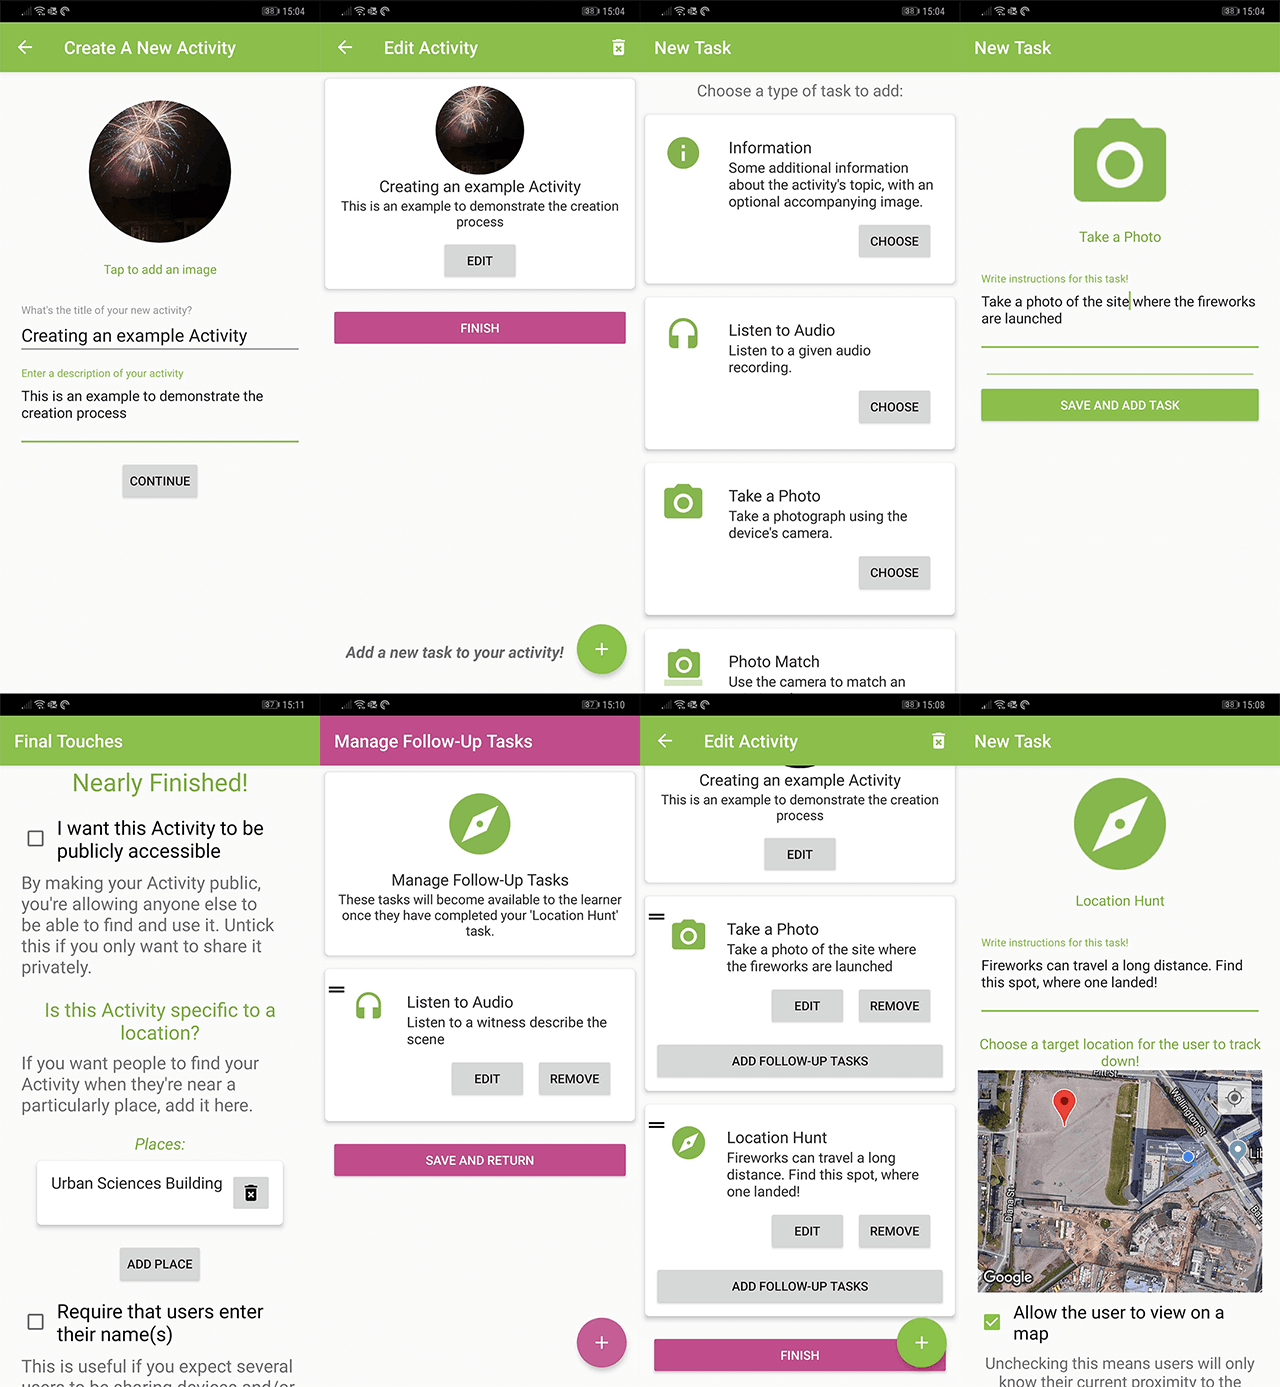
\includegraphics[width=1\columnwidth]{images/chapter05/creation.png}
  \caption[Creating an OurPlace activity]{Creating an OurPlace activity (clockwise, from top left): a) Choosing the activity's title, description and image; b) The Activity overview screen; c) Choosing a Task Type to add; d) Adding a basic \textit{Take a Photo} Task, with a description, e) Adding a more complicated \textit{Location Hunt} Task, with description and target coordinates; f) The new Tasks in the Activity overview; g) Adding Follow-Up Tasks to the \textit{Location Hunt}; h) The final touches before uploading }~\label{fig:ActivityCreation}
\end{figure*}

\subsection{Sharing, Discovering and Launching Activities}
\label{sec:SharingActivities}

\subsubsection{The Highlights Feed and Location}

\subsubsection{Share Codes and QR Codes}

\section{Implementation of the OurPlace Mobile Applications}
\label{sec:ImplementationMobile}

\subsection{Improvements over ParkLearn}

\subsubsection{Developing the iOS Application}

\subsubsection{Adding Follow-Up Tasks}

\subsubsection{QR Code Task Types}

\subsubsection{Other General Improvements}


\subsection{The OurPlace App}

\section{Implementation of the API and Website}
\label{sec:ImplementationWeb}

\section{Development of the Technology}

\subsection{Why use the Xamarin framework?}
The OurPlace platform is a system consisting of smartphone applications for the
Android and iOS (Apple iPhone and iPad) operating systems, a website and an
online application programming interface (API). It was decided that in order to
support as many schools, groups and individuals as possible, both of the main
smartphone OSs should be supported (Android and iOS). Furthermore, in order to
provide a high quality experience which conformed to each platform's expected
design metaphors,  supported access to all of the devices' hardware features and
didn't require a constant internet connection, I decided to produce `native'
applications for each platform (that is, rather than produce something like a
website which would be the same across all platforms). Ordinarily, this would
result in having to produce software in multiple programming languages: for
example, Android applications are usually written in either Java or Kotlin,
whereas iPhone apps are written in Objective-C, which is very different. As the
project was mostly a one-man show, dedicating large amounts of time to learning,
developing, iterating and maintaining systems across multiple languages was
unrealistic. 

In the end, the decision was made to develop the mobile applications using the
Xamarin framework. This framework takes code written in C\# and compiles it into
`native' applications, meaning that apps look, feel and act like software
written in the different platforms' specific languages. This gave the advantage
of sharing the same programming language across both applications, without
losing out on any major features and allowing for common code (functionality
identical across the two applications, e.g. making requests to the server) to be
shared across the projects. To fully capitalise on this code sharing advantage,
it was decided to take this further and produce the website and API in C\#. As a
result, every component of the OurPlace platform can be opened within the same
Visual Studio `solution', significantly speeding up the development process.

\subsection{Disadvantages to using Xamarin}
While developing the mobile applications with the Xamarin framework
significantly reduced to upfront time investment in the development process, it
certainly had its trade-offs which became more apparent as the project grew.
Having all of the OurPlace code available within one solution (discussed in
\ref{sec:OurPlaceSolution}) was certainly convenient and minimised code
duplication, but when combined with Xamarin's more demanding build process it
created large performance overheads. This, combined with issues of documentation
being in other programming languages (particularly on the iOS application),
impeded the development workflow, frequently slowing it to a crawl. At the end
of the project, it is difficult to say if significant time was saved by using
Xamarin over the two platforms' `native' development tools. However, anyone
considering these options should note that recent developments to Visual Studio
and the Xamarin framework have significantly improved performance, which may somewhat
mitigate these issues.

\subsection{A Brief Tour of the OurPlace Visual Studio Solution}
\label{sec:OurPlaceSolution}
All of the OurPlace code is open source, and can be viewed at
\url{https://github.com/GSDan/OurPlace}. Using C\# and Microsoft's .NET Framework
across the OurPlace platform afforded it being accessible within a single Visual
Studio solution, split into four smaller component projects:
\textit{OurPlace.Common}, \textit{OurPlace.API}, \textit{OurPlace.Android} and
\textit{OurPlace.iOS}.

\paragraph{OurPlace.Common}
This is a .NET Standard 2.0 project, which acts as a `library' of functions and
serves the other projects within the solution. It contains shared data models,
interfaces and common core functionality, including managing the apps' local
files, authenticating with the server, polling it for the latest OurPlace
activities and uploading new activities and responses. This is the only project
which is referenced from elsewhere in the solution.

\paragraph{OurPlace.API}
This project uses version 4.6.1 of the .NET Framework, and contains an ASP .NET
website, a Web API 2 powered API and a Code First, Entity Framework database.
This project is discussed in detail in section \ref{sec:ImplementationWeb}.

\paragraph{OurPlace.Android}
This project contains all of the code specific to the Android application.
Written in C\# using the Xamarin.Android framework, a `native' Android application is
produced upon compilation, supporting devices running Android versions as old as
4.1 (Jelly Bean, 2012) and targeting the latest features found in version 8.1
(Oreo, 2017). This project is discussed in detail in section
\ref{sec:ImplementationMobile}.

\paragraph{OurPlace.iOS}
This project contains all of the code specific to the iPhone/iPad application.
Written in C\# using the Xamarin.iOS framework, a `native' iOS application is
produced upon compilation. The application requires a minimum of iOS 10, which
is supported by devices as old as the iPhone 5 (released 2012). This project is
discussed in detail in section \ref{sec:ImplementationMobile}.